\documentclass{report}

\usepackage[margin=1in]{geometry}
\usepackage{amsmath}
\usepackage{graphicx}



\title{Access to Food in Chicago: \\ a Hierarchical Perspective}
\author{Daniel Berry}

\begin{document}

\maketitle

\begin{abstract}
  Easy access to healthy, nutrient rich foods is a current public health crisis in the United States. Areas that have limited access to healthy foods and easy access to unhealthy foods are called ``food deserts''.  %TODO: citation
  In the United States today, X million people are living in a food desert. %TODO: citation
  Access to food can be measured at the city-block level and can have substantial variation within a single neighborhood. However, much publicly available city wide health data is available at the neighborhood level. This gives the data a natural hierarchical structure as city blocks are nested within neighborhoods. In this paper we model presence/absence of deserts using a combination of block-level and neighborhood-level data from the city of Chicago. We apply construct a hierarchical logistic regression model and demonstrate its superiority. 
\end{abstract}


\section*{Introduction}
Access to readily available and inexpensive healthy food options is important for personal health. Unfortunately, for some in society today, access is not equitable. Some towns and neighborhoods have excellent healthy food options. Others do not. In some locations it is difficult to impossible for many residents to find healthy food options. In these areas, known as food deserts, there is readily available processed, calorie dense but nutrient poor foods.

A person's access to food is determined by the city block in which they live. Any increase in precision beyond the city block level is meaningless. However, rarely is data reported at the city block level. Sampling variability at that level would make drawing conclusions difficult. For that and other reasons, often city data is reported at the neighborhood, zip code, or telephone area code level. This gives the data a natural hierarchical structure where city blocks are nested within neighborhoods. 

\subsection*{Food Deserts}
There is no single agreed upon definition of a food desert. Some common metrics are based on distances to nearest supermarket with cutoffs at 1 mile for urban areas and 10 miles for rural areas. 1 mile may seem like a short distance to travel, but in urban areas with low car ownership rates where residents rely on public transportation, a 1 mile journey can take a substantial amount of time. 
% TODO: insert citation
For this work we used the definition from %TODO: citation
of defining a city block as being in a food desert if the city block is more than 1 mile from a supermarket. Supermarket in this context is a grocery store that is larger than 10000 square feet %TODO: citation
that is not primarily a liquor store. Distance is defined as the great circle distance from the center of mass of the city block to the center of mass of the grocery store.

We can see the location of food deserts as computed using our metric visualized in figure \ref{fig:desert}. 
\begin{figure}[h!]
  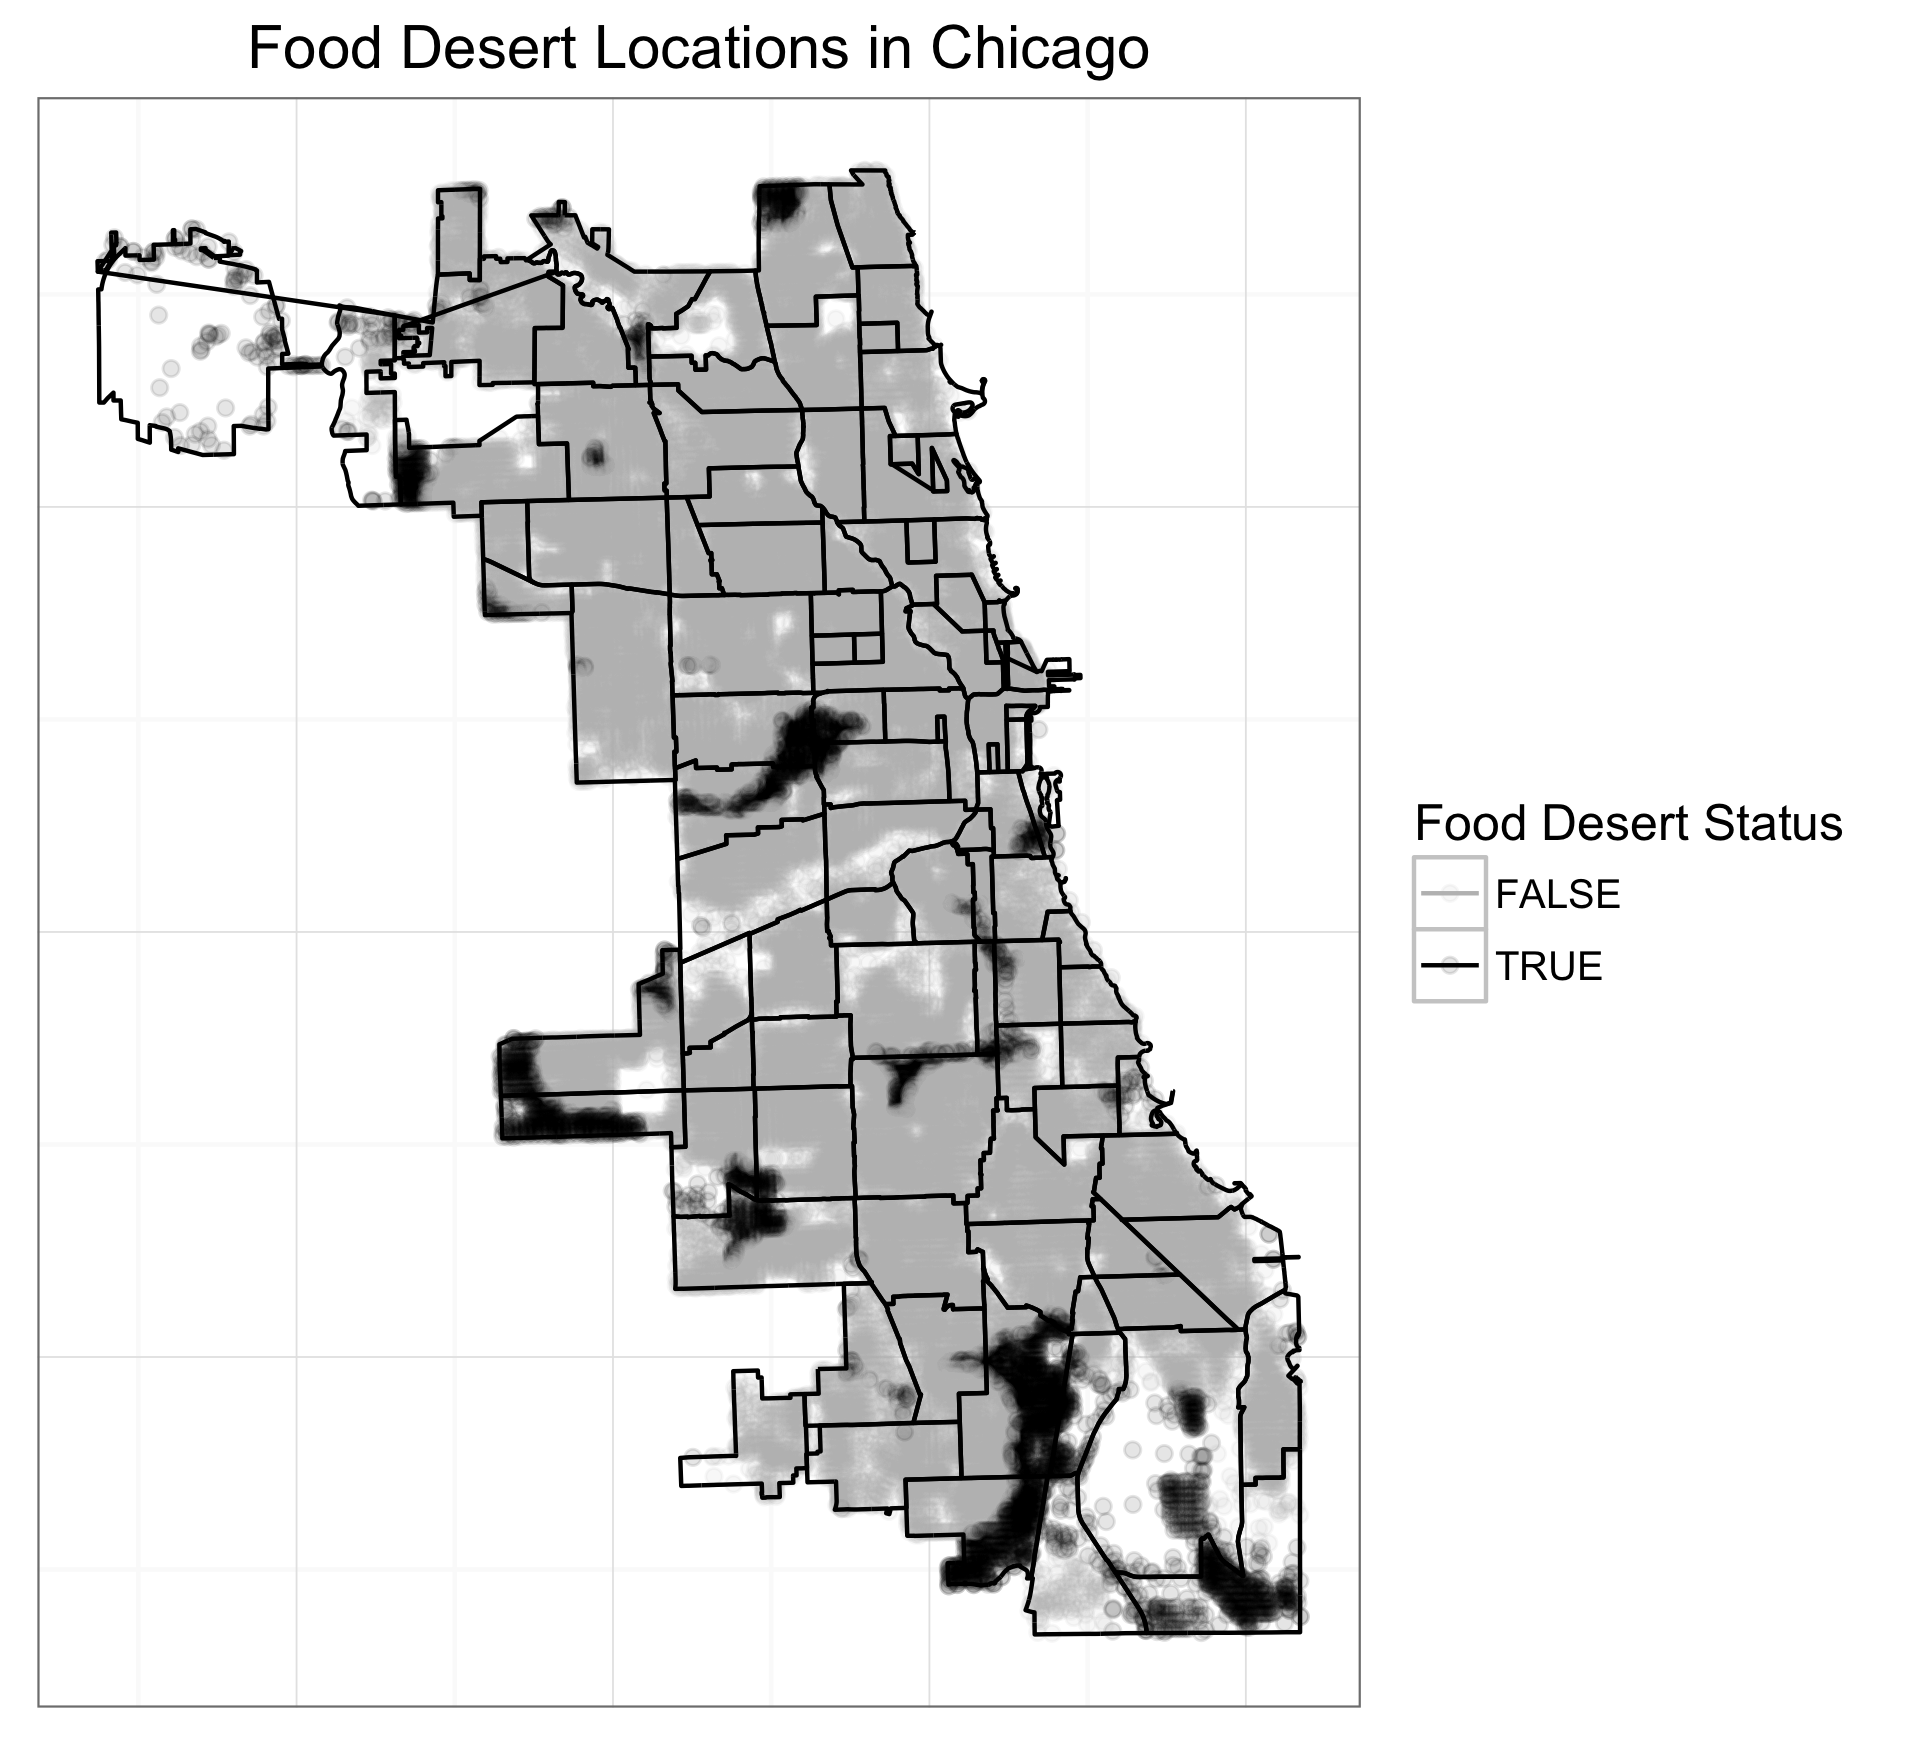
\includegraphics[scale=.2]{deserts_plot}
  \caption{Food Desert Locations in Chicago}
  \label{fig:desert}
\end{figure}

Chicago is a very racially segregated city. As shown in figures \ref{fig:black} and \ref{fig:white}, many neighborhoods in Chicago are $>$75\% a single race.

\begin{figure}[h!]
  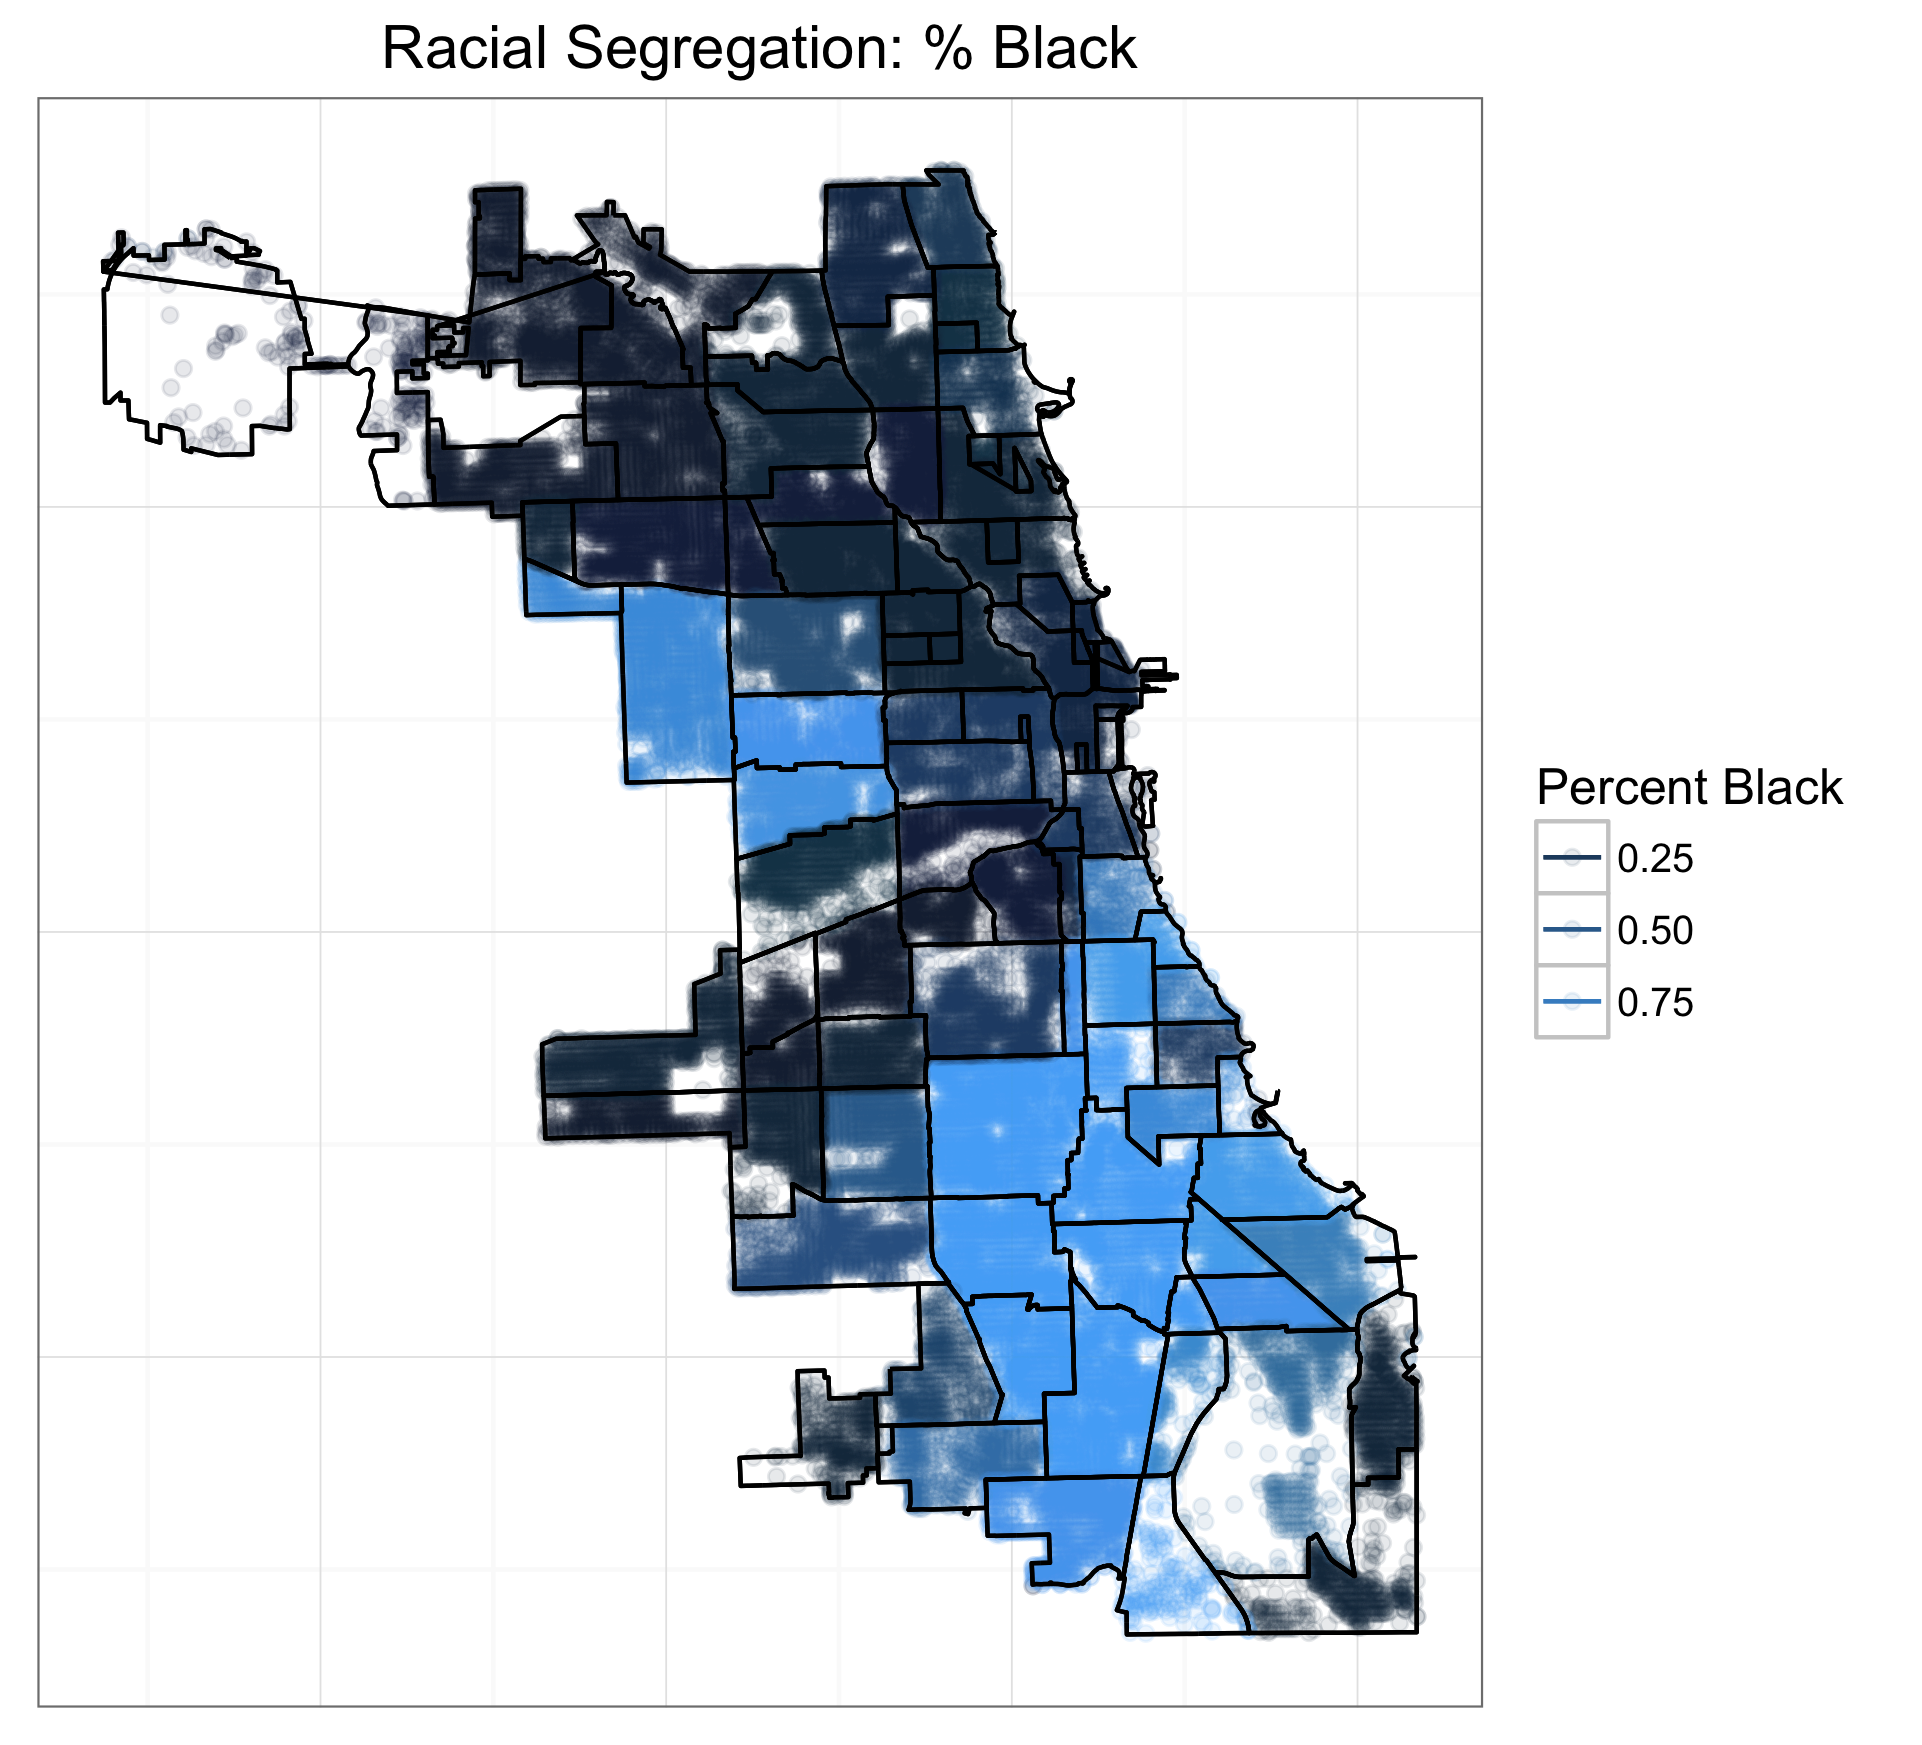
\includegraphics[scale=.2]{pct_black_plot}
  \caption{Neighborhoods by Black Percentage}
  \label{fig:black}
\end{figure}

\begin{figure}[h!]
  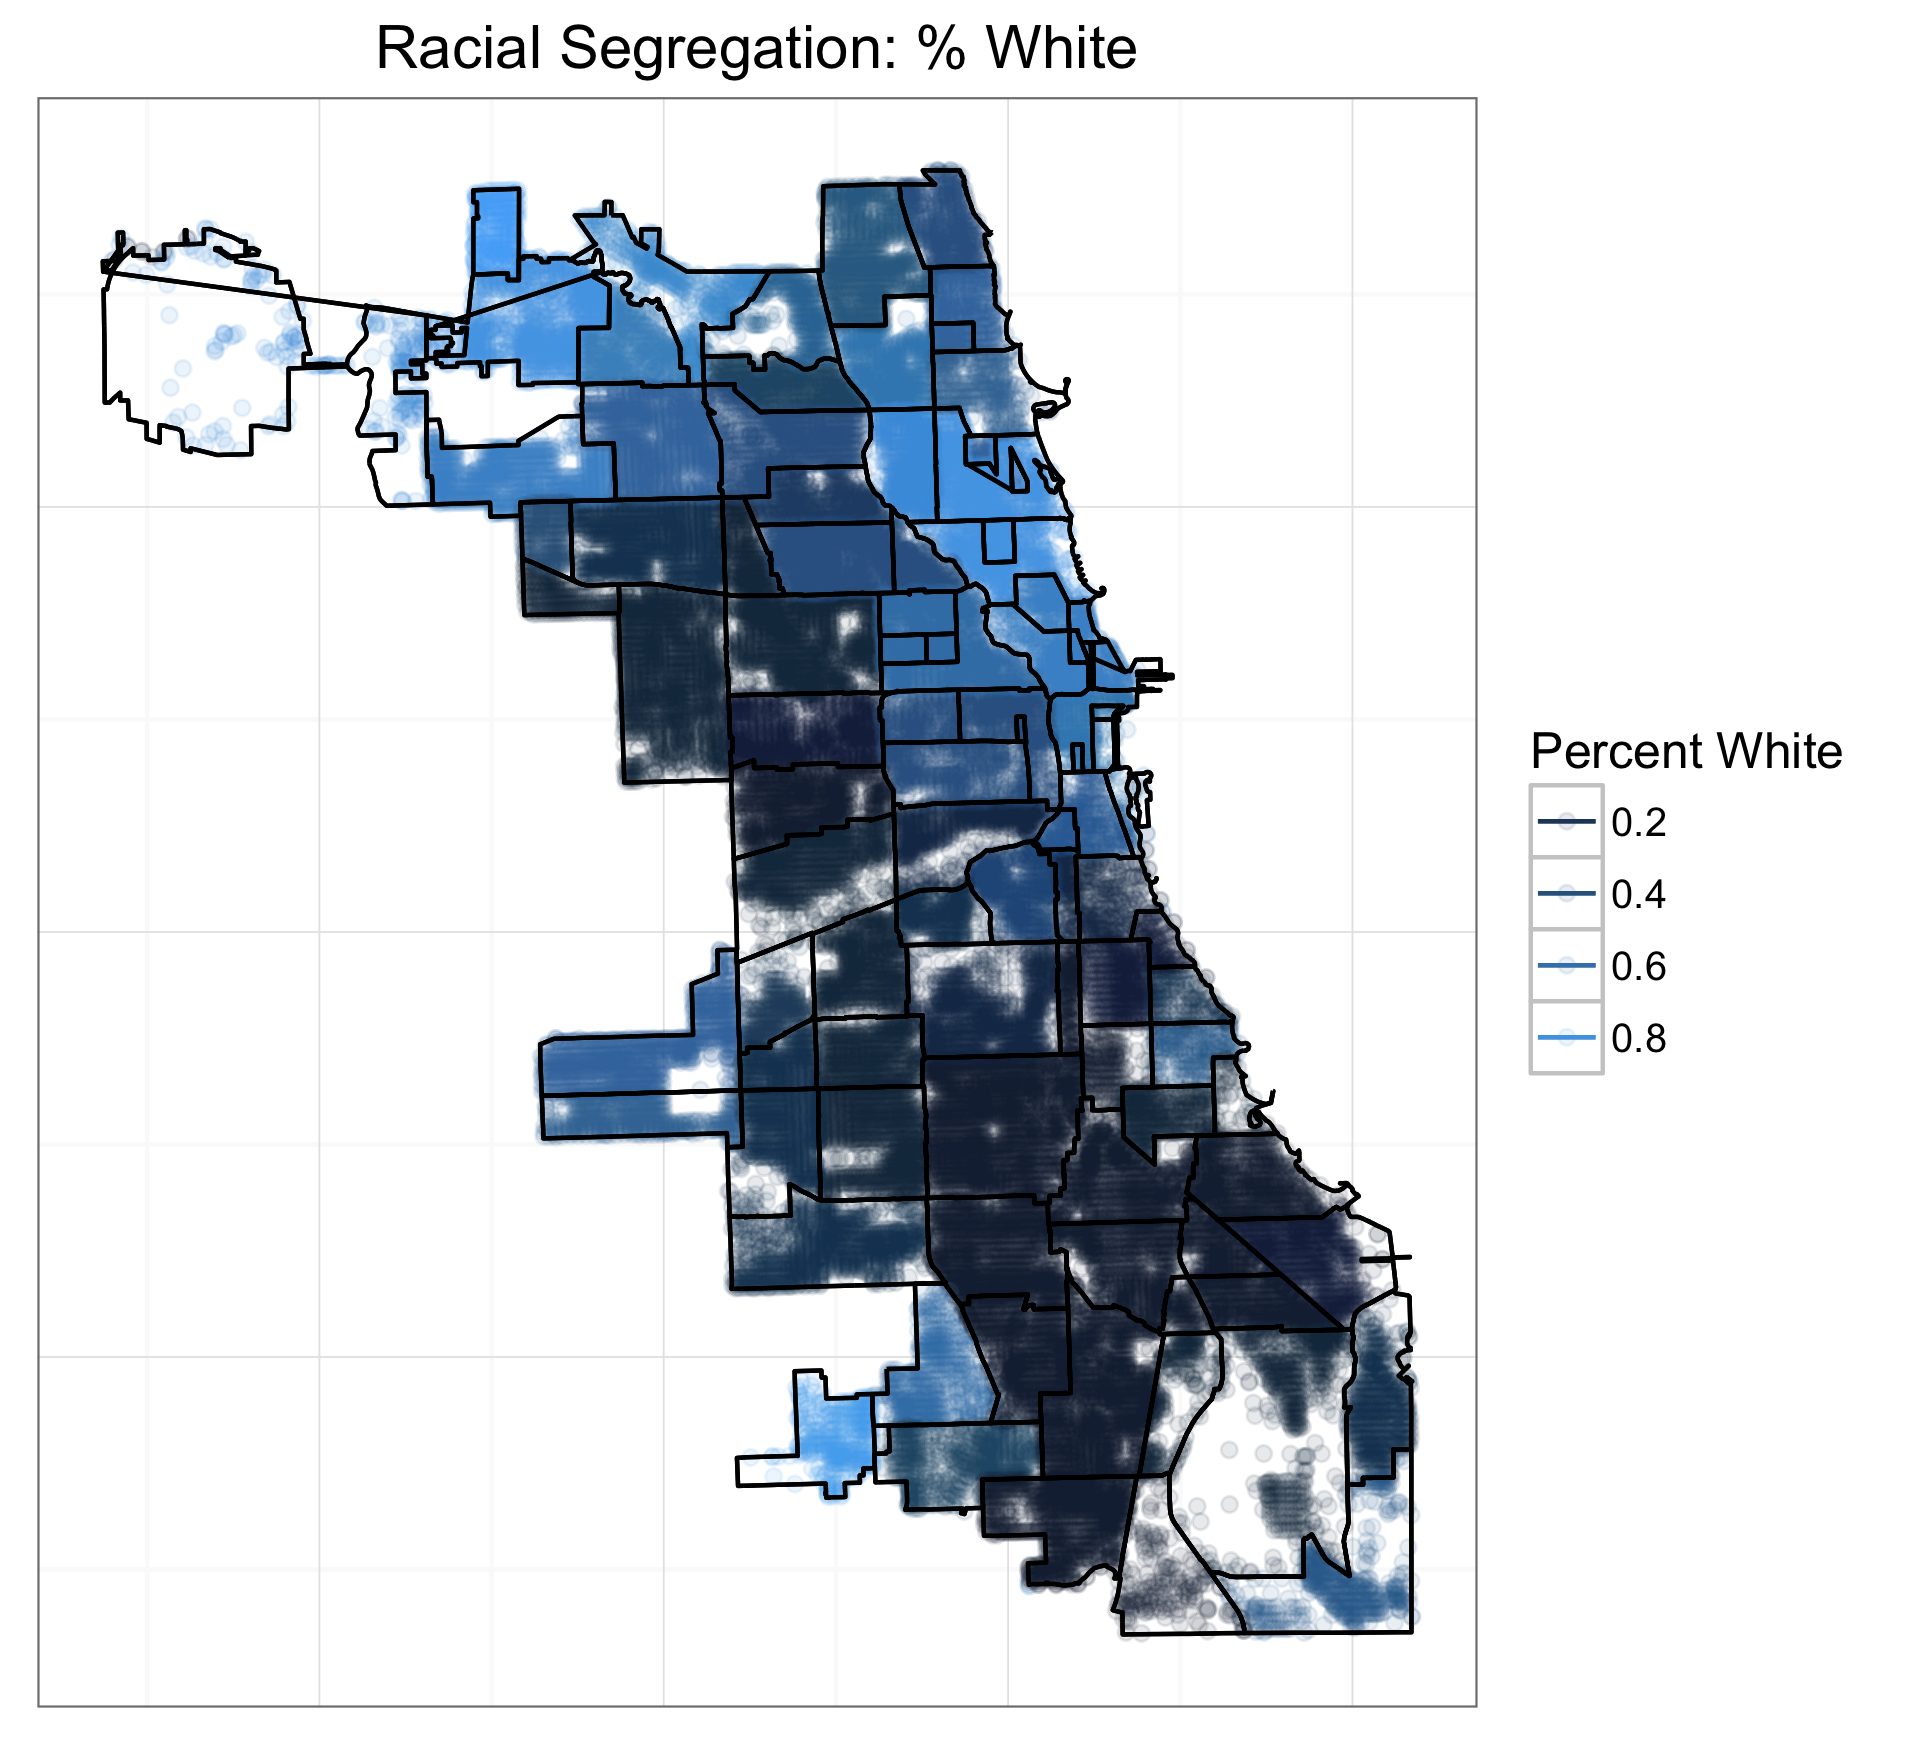
\includegraphics[scale=.2]{pct_white_plot}
  \caption{Neighborhoods by White Percentage}
  \label{fig:white}
\end{figure}

In fact, it appears that many food deserts are located in majority black neighborhoods. We will explore this relationship later on during the model building phase. Chicago also has very strong class divisions. For example the (near) north side is very wealthy while the south side and suburbs are less so,  see \ref{fig:income}. 

\begin{figure}[h!]
  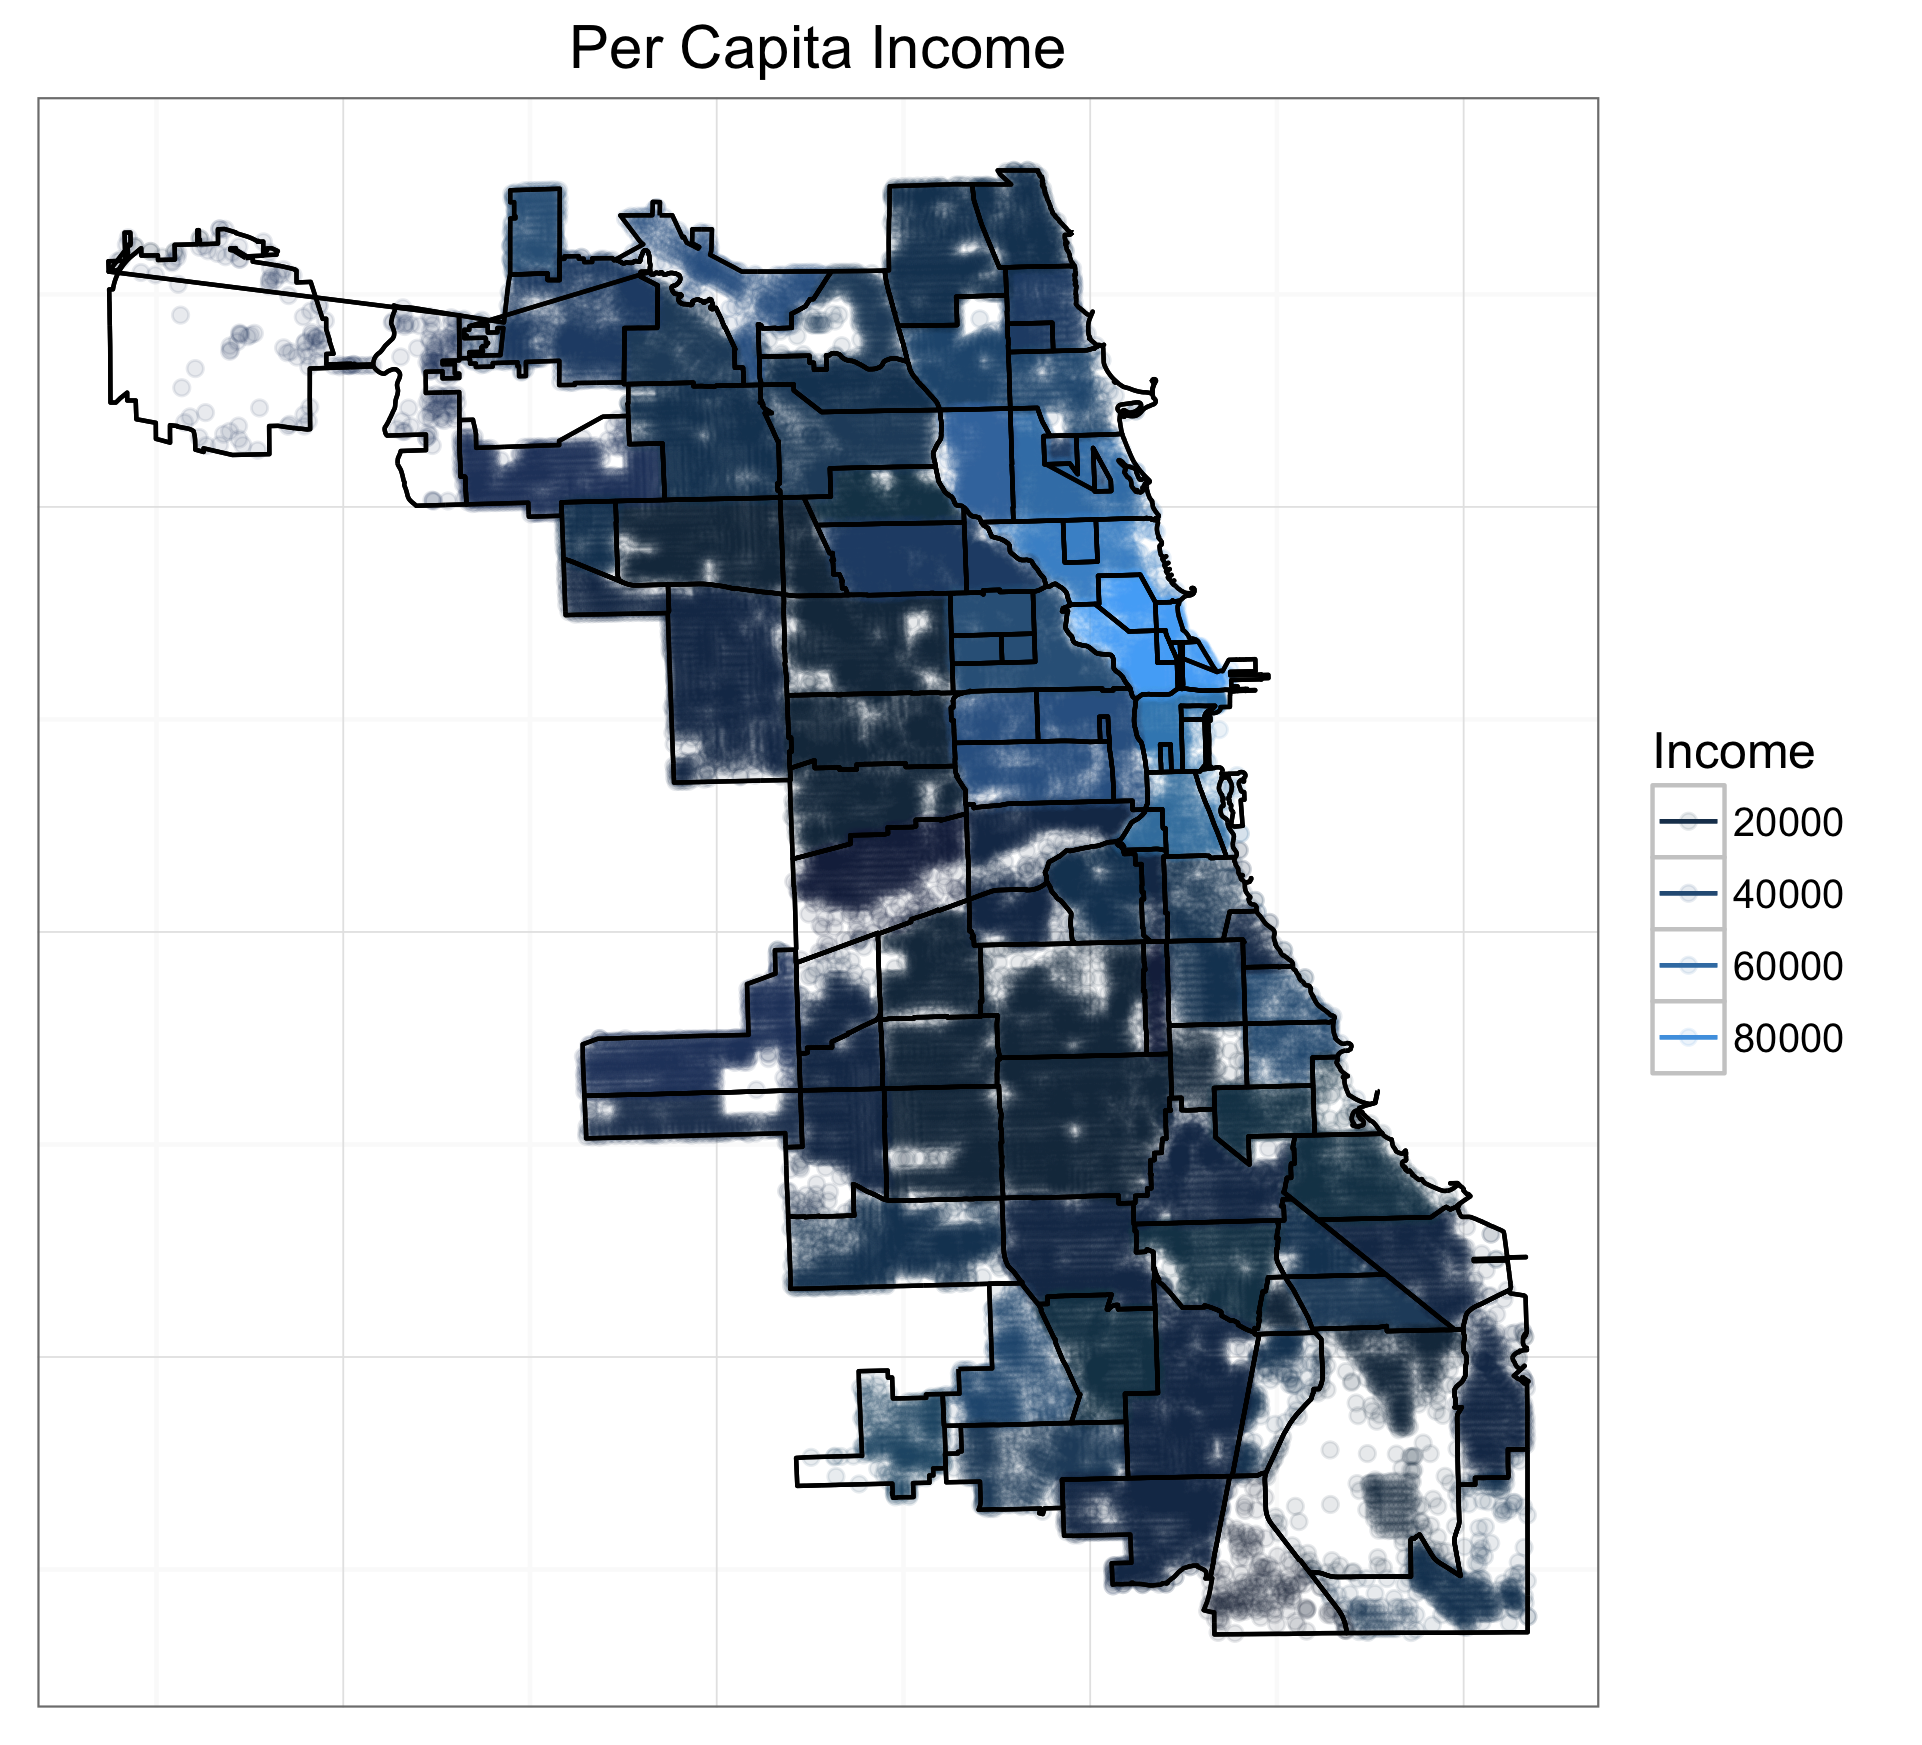
\includegraphics[scale=.2]{income_plot}
  \caption{Neighborhoods by Per Capita Income}
  \label{fig:income}
\end{figure}

Perhaps instead, food deserts are associated with urban decay. We might hypothesize that 

\begin{figure}[h!]
  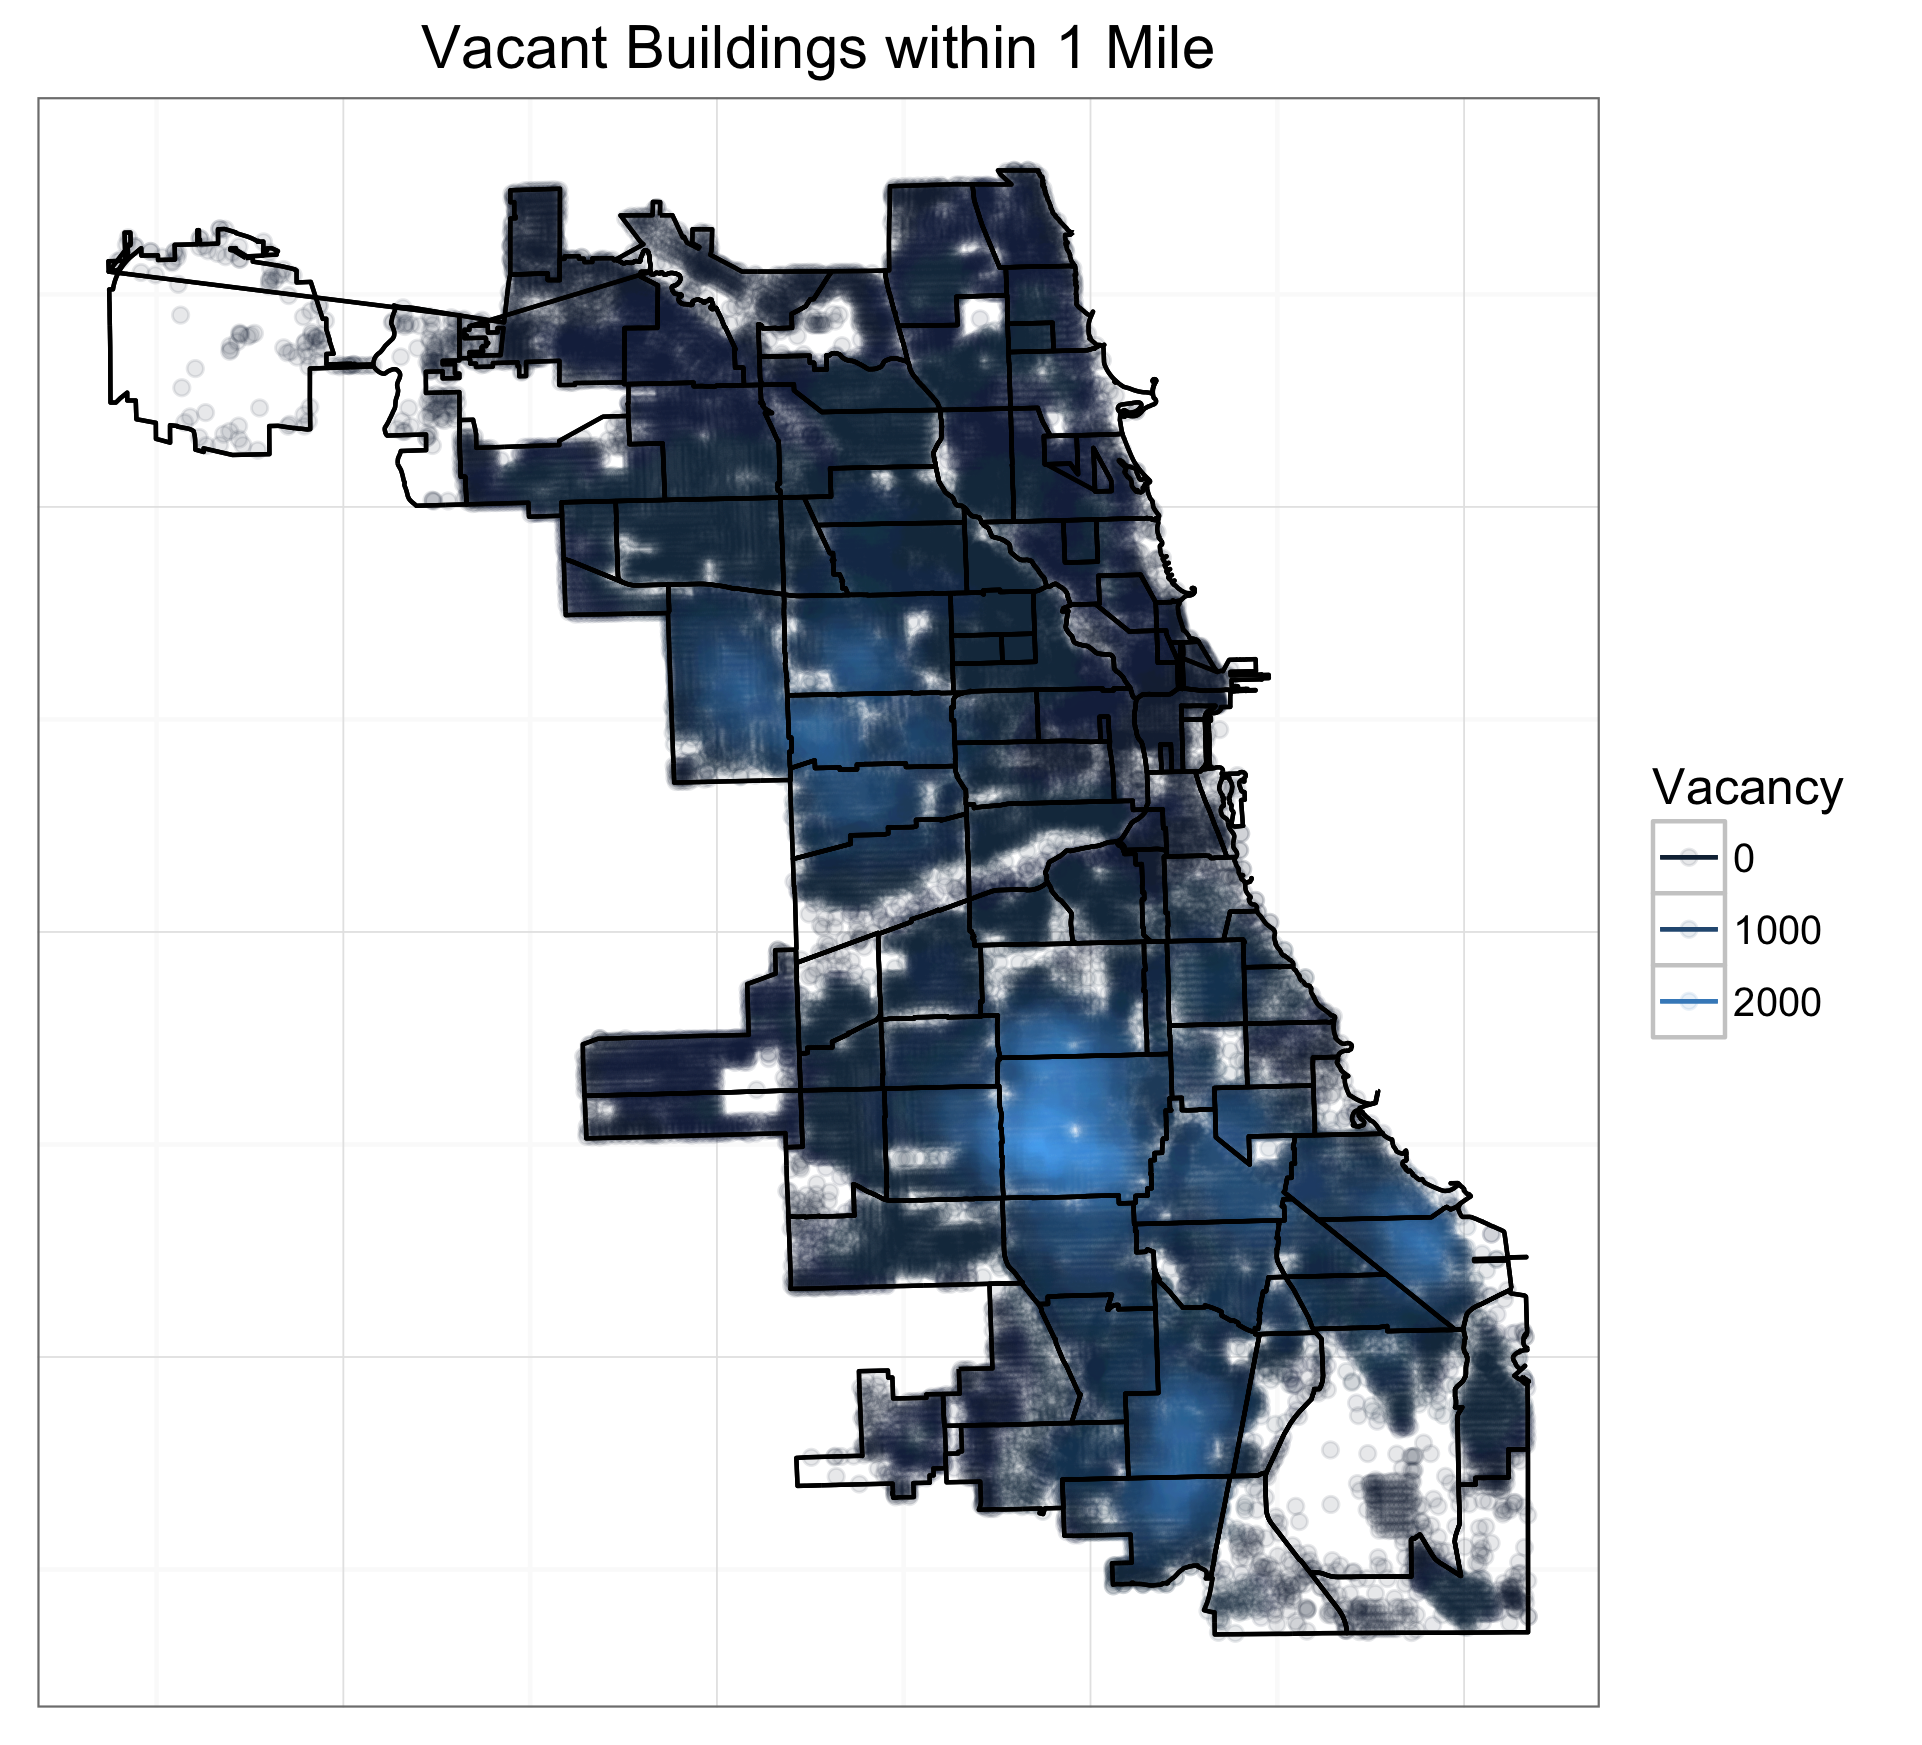
\includegraphics[scale=.2]{vacant_plot}
  \caption{Neighborhoods by Number Vacant Buildings with 1 Mile Radius}
  \label{fig:vacant}
\end{figure}


\section*{Methods}
In the following section we describe the procedures used. We begin by describing the data used and including data sources. Then we move on to describing the types of models used. 

\subsection*{Data Gathering and Manipulation}

All data was sourced from the generous Open Data Portal operated by the city of Chicago. The portal can be found at data.cityofchicago.org. We utilized the following data files:

\subsubsection*{Block level data}

\paragraph{ Crimes 2001 - present}
This file contains a record for crimes in Chicago since 2001 with information about the type of crime as well as its location. The location is pseudo-anonymized to be random but within the same city block. For each city block we counted the total number of crimes committed within 1 mile in 2009. Our hypothesis \textit{a priori} was that food deserts were often located in high-crime areas.


\paragraph{ 311 Service Requests: Vacant Buildings}
This file contains a record for every 311 service call about an abandoned/unoccupied/unlawfully occupied building. For each city block we counted the number of calls for vacant buildings where the building was located within 1 mile of the city block. Our hypothesis was that food deserts were located in areas with higher levels of vacant buildings. 

\paragraph{ CTA Ridership: Avg. Weekly Boardings during October 2010}
This file contains average weekly boardings for the month of October 2010 for every CTA (Chicago Transit Authority) bus stop in Chicago. We counted the total boardings for all stops within a mile of each city block. Our hypothesis was that residents of food deserts would tend to have a higher reliance on public transportation than residents in other areas. 

\paragraph{ Census Block Population  }
This file contains the population of each city block. 

\subsubsection*{Neighborhood level data}

\paragraph{ Public Health Statistics: selected public health indicators by Chicago community area}
This file contains a record for every neighborhood in Chicago with selected public health information. Examples include teenage births per 100,000 residents and Gonorrhea prevelence (cases per 100,000). Our hypothesis was that food deserts were likely to be underserved in a more general public health sense than just lacking access to food. 

\paragraph{ Census Data: Selected socioeconomic indicators    }
This file contains a record for every neighborhood in Chicago with information about the socioeconomic status of that neighborhood. Examples include percent of residents below the povery level and percent without a high school diploma. 

\paragraph{ Race by Community Area }
This file contains a record for every neighborhood in Chicago with the number of residents of each race who reside in that neighborhood. \\

We tried to gather data on crimes and use that information in the model, however the available dataset for crimes in chicago is rather large ($>$1 GB) and we didn't have time to finish extracting features from that model. We hypothesized that food deserts were more likely to be in high crime areas. 

\subsection*{Generalized Linear Models}

In ordinary linear regression (or ordinary least squares, OLS) we assume that our observations $y$ are some linear combination of the covariates, $x_i$'s that we have plus random error. In matrix notation this can be expressed as: $$y = X\beta + \epsilon$$ where $y$ is the vector of responses, $X$ is the (model) matrix of data, $\beta$ is the vector of regression coefficients, and $\epsilon \sim N(0, \sigma^2 I)$ is the random error.

Generalized linear models extends this to non-normally distributed responses through the use of a link function $g$: $$Y = g^{-1}(X\beta)$$. For {0,1} or binomially distributed responses, there are a variety of link functions available. One of the most common is the logit link: $g(x) = \log(\frac{x}{1-x})$. For simplicity, we chose the logit link although there are certainly other options available (probit, t, etc.). 

\subsection*{Mixed Models}

So far we have discussed models which have only ``fixed effects'', that is, effects that are nonrandom and do not vary across covariates. We may believe for example that each neighborhood is different enough to merit its own intercept but that each neighborhood is sampled from a large population of candidate neighborhoods. In that situation we're not interested necessarily in each intercept, but more the variability between neighborhoods. In this situation we would fit a random intercept model where each intercept is (without loss of generality) distributed normally with mean zero and variance $\sigma^2_\alpha$.  To further generalize, we could allow the fixed effect coefficients to vary in a similar manner. This is called a random slope model. In our case we fit random intercept models with fixed effects for each slope. This reflects our belief that the neighborhoods are different from each other and should have different baseline probabilities of being a food desert (due to potentially unmeasured covariates) but that the effect of CTA ridership and number of vacant buildings nearby should be the same across all neighborhoods. 

\subsection*{Hierarchical Models}

Hierarchical models are another extension to the family of linear models which allow for hierarchical structured data. Recalling the random intercept model, since we have neighborhood level covariates, we would like to use the information contained within to predict the random intercept for each neighborhood. 
\subsection*{Models Fit}

\subsubsection*{Complete Pooling}

To begin we have the simplest model: ordinary regression using only the block-level variables. This model pools together every neighborhood as if the neighborhood distinctions don't matter. 

$$ y_{ij} = \text{logit}^{-1}\left( \alpha + X_{B}\beta_{B} + \epsilon_{ij} \right) $$

Where $\epsilon_{ij} \sim N(0, \sigma^2)$

\subsubsection*{No Pooling}

The next model has a different but nonrandom intercept for each neighborhood, a fixed effect for that neighborhood. This would correspond to our belief that the neighborhoods are each different from the others. 

$$ y_{i} = \text{logit}^{-1}\left( \alpha + X_{B}\beta_{B} +  \gamma_j + \epsilon_{ij} \right) $$

Where $\epsilon_i \sim N(0, \sigma^2)$ 

\subsubsection*{Partial pooling}

The next model has a random intercept for each neighborhood which corresponds to partially pooling the data together. For every neighborhood we use some of the information in other neighborhoods to estimate its intercept. That is, the intercepts in the previous model are shrunk toward the common mean. 

$$ y_{i} = \text{logit}^{-1}\left( \alpha_{j[i]} + X_{B}\beta_{B} +  \epsilon_i \right) $$

Where $\epsilon_i \sim N(0, \sigma^2)$ and $\alpha_j \sim N(0, \sigma^2_\alpha)$

\subsubsection*{Hierarchical}

The final and most complicated model that was fit was a hierarchical model including the neighborhood level predictors in estimating the random intercept for each neighborhood. 

$$ y_{i} = \text{logit}^{-1}\left( \alpha_{j[i]} + X_{B}\beta_{B} +  \epsilon_i \right) $$

Where $\epsilon_i \sim N(0, \sigma^2)$ and $\alpha_j \sim N(X_N \beta_N, \sigma^2_\alpha)$


\subsection*{Model Comparison}

Models were compared using AIC and cross validated Breir Score (Mean Square Error in the case of 2-class logistic regression). Lower values of AIC indicate better fitting models and thus can be used to compare the performance of models to each other. The cross validation was performed 10 fold where the model was fit on 80\% of the data (sampled in a stratified manner based on Neighborhood) and evaluated on the remaining 20\%. This gives a way of quantifying the predictive ability of the model on new, unseen city blocks. . 

\section*{Results}

\subsection*{Model Parameters}

\subsubsection*{Complete Pooling}

% % Table created by stargazer v.5.2 by Marek Hlavac, Harvard University. E-mail: hlavac at fas.harvard.edu
% % Date and time: Mon, Nov 21, 2016 - 10:52:26
% \begin{table}[!htbp] \centering 
%   \caption{Complete pooling model summary} 
%   \label{cpresult} 
% \begin{tabular}{@{\extracolsep{5pt}}lc} 
% \\[-1.8ex]\hline 
% \hline \\[-1.8ex] 
%  & \multicolumn{1}{c}{\textit{Dependent variable:}} \\ 
% \cline{2-2} 
% \\[-1.8ex] & desert \\ 
% \hline \\[-1.8ex] 
%  CTA\_counts & $-$1.585$^{***}$ (0.040) \\ 
%   & \\ 
%  vacant\_counts & 0.411$^{***}$ (0.018) \\ 
%   & \\ 
%  Constant & $-$2.848$^{***}$ (0.028) \\ 
%   & \\ 
% \hline \\[-1.8ex] 
% Observations & 36,870 \\ 
% Log Likelihood & $-$9,913.778 \\ 
% Akaike Inf. Crit. & 19,833.560 \\ 
% \hline 
% \hline \\[-1.8ex] 
% \textit{Note:}  & \multicolumn{1}{r}{$^{*}$p$<$0.1; $^{**}$p$<$0.05; $^{***}$p$<$0.01} \\ 
% \end{tabular} 
% \end{table}

% Table created by stargazer v.5.2 by Marek Hlavac, Harvard University. E-mail: hlavac at fas.harvard.edu
% Date and time: Mon, Nov 21, 2016 - 13:53:33
\begin{table}[!htbp] \centering 
  \caption{Complete pooling model summary} 
  \label{cpresult} 
\begin{tabular}{@{\extracolsep{5pt}}lc} 
\\[-1.8ex]\hline 
\hline \\[-1.8ex] 
 & \multicolumn{1}{c}{\textit{Dependent variable:}} \\ 
\cline{2-2} 
\\[-1.8ex] & desert \\ 
\hline \\[-1.8ex] 
 CTA\_counts & $-$1.588$^{***}$ (0.040) \\ 
 vacant\_counts & 0.410$^{***}$ (0.018) \\ 
 crime & 0.056$^{***}$ (0.019) \\ 
 Constant & $-$2.849$^{***}$ (0.029) \\ 
\hline \\[-1.8ex] 
Observations & 36,870 \\ 
Log Likelihood & $-$9,909.356 \\ 
Akaike Inf. Crit. & 19,826.710 \\ 
\hline 
\hline \\[-1.8ex] 
\textit{Note:}  & \multicolumn{1}{r}{$^{*}$p$<$0.1; $^{**}$p$<$0.05; $^{***}$p$<$0.01} \\ 
\end{tabular} 
\end{table} 

\subsubsection*{No Pooling}

% % Table created by stargazer v.5.2 by Marek Hlavac, Harvard University. E-mail: hlavac at fas.harvard.edu
% % Date and time: Mon, Nov 21, 2016 - 10:52:50
% \begin{table}[!htbp] \centering 
%   \caption{No pooling model summary} 
%   \label{npresult} 
% \begin{tabular}{@{\extracolsep{5pt}}lc} 
% \\[-1.8ex]\hline 
% \hline \\[-1.8ex] 
%  & \multicolumn{1}{c}{\textit{Dependent variable:}} \\ 
% \cline{2-2} 
% \\[-1.8ex] & desert \\ 
% \hline \\[-1.8ex] 
%  CTA\_counts & $-$0.783$^{***}$ (0.061) \\ 
%  vacant\_counts & $-$0.408$^{***}$ (0.038) \\ 
%  NeighborhoodArcher Heights & $-$0.379 (1,446.793) \\ 
%  NeighborhoodArmour Square & 17.949 (757.683) \\ 
%  NeighborhoodAshburn & 18.311 (757.683) \\ 
%  NeighborhoodAuburn Gresham & 14.135 (757.683) \\ 
%  NeighborhoodAustin & 16.948 (757.683) \\ 
%  NeighborhoodAvalon Park & 16.015 (757.683) \\ 
%  NeighborhoodAvondale & 0.466 (1,120.896) \\ 
%  NeighborhoodBelmont Cragin & $-$0.232 (951.136) \\ 
%  NeighborhoodBeverly & 16.982 (757.683) \\ 
%  NeighborhoodBridgeport & 16.182 (757.683) \\ 
%  NeighborhoodBrighton Park & $-$0.294 (1,090.129) \\ 
%  NeighborhoodBurnside & $-$0.020 (2,106.584) \\ 
%  NeighborhoodCalumet Heights & 15.497 (757.683) \\ 
%  NeighborhoodChatham & 17.624 (757.683) \\ 
%  NeighborhoodChicago Lawn & 17.597 (757.683) \\ 
%  NeighborhoodClearing & 20.147 (757.683) \\ 
%  NeighborhoodDouglas & 0.264 (1,789.225) \\ 
%  NeighborhoodDunning & 18.404 (757.683) \\ 
%  NeighborhoodEast Side & $-$0.950 (1,160.930) \\ 
%  NeighborhoodEdgewater & 0.290 (1,092.033) \\ 
%  NeighborhoodEdison Park & 16.367 (757.683) \\ 
%  NeighborhoodEnglewood & 19.683 (757.683) \\ 
%  NeighborhoodForest Glen & 17.800 (757.683) \\ 
%  NeighborhoodFuller Park & 18.461 (757.683) \\ 
%  NeighborhoodGage Park & $-$0.038 (1,116.702) \\ 
%  NeighborhoodGarfield Park & 20.416 (757.683) \\ 
%  NeighborhoodGarfield Ridge & 18.375 (757.683) \\ 
%  NeighborhoodGrand Boulevard & 18.233 (757.683) \\ 
%  NeighborhoodGreater Grand Crossing & 1.174 (1,060.103) \\ 
%  NeighborhoodHegewisch & 22.019 (757.683) \\ 
%  NeighborhoodHermosa & $-$0.097 (1,318.741) \\ 
%  NeighborhoodHumboldt Park & 14.379 (757.683) \\ 
%  NeighborhoodHyde Park & 0.320 (1,585.606) \\ 
%  NeighborhoodIrving Park & $-$0.045 (1,000.878) \\ 
%  NeighborhoodJefferson Park & $-$0.628 (1,084.084) \\ 
%  NeighborhoodKenwood & 0.139 (1,833.318) \\ 
%  NeighborhoodLake View & 0.553 (997.500) \\ 
%  NeighborhoodLincoln Park & 0.295 (1,091.797) \\ 
%  NeighborhoodLincoln Square & 0.151 (1,086.733) \\ 
%  NeighborhoodLogan Square & 0.368 (928.968) \\ 
%  NeighborhoodLoop & 4.566 (1,622.709) \\ 
%  NeighborhoodLower West Side & $-$0.194 (1,142.009) \\ 
%  NeighborhoodMcKinley Park & $-$0.442 (1,387.487) \\ 
%  NeighborhoodMontclaire & $-$0.641 (1,429.041) \\ 
%  NeighborhoodMorgan Park & 14.297 (757.683) \\ 
%  NeighborhoodMount Greenwood & $-$1.030 (1,241.482) \\ 
%  NeighborhoodNear North Side & 1.297 (1,065.341) \\ 
%  NeighborhoodNear South Side & 0.223 (1,645.912) \\ 
%  NeighborhoodNear West Side & 19.805 (757.683) \\ 
%  NeighborhoodNew City & 17.535 (757.683) \\ 
%  NeighborhoodNorth Center & 0.027 (1,073.236) \\ 
%  NeighborhoodNorth Lawndale & 20.141 (757.683) \\ 
%  NeighborhoodNorth Park & $-$0.525 (1,315.485) \\ 
%  NeighborhoodNorwood Park & 15.844 (757.683) \\ 
%  NeighborhoodO'Hare & 17.370 (757.683) \\ 
%  NeighborhoodOakland & $-$0.346 (2,337.413) \\ 
%  NeighborhoodPortage Park & 17.008 (757.683) \\ 
%  NeighborhoodPullman & 20.484 (757.683) \\ 
%  NeighborhoodRiverdale & $-$0.904 (2,643.084) \\ 
%  NeighborhoodRogers Park & $-$0.162 (1,141.035) \\ 
%  NeighborhoodRoseland & 21.120 (757.683) \\ 
%  NeighborhoodSouth Chicago & 0.467 (1,066.990) \\ 
%  NeighborhoodSouth Deering & 18.453 (757.683) \\ 
%  NeighborhoodSouth Lawndale & $-$0.081 (1,038.677) \\ 
%  NeighborhoodSouth Shore & 14.922 (757.683) \\ 
%  NeighborhoodUptown & 0.818 (1,290.791) \\ 
%  NeighborhoodWashington Heights & 17.330 (757.683) \\ 
%  NeighborhoodWashington Park & 19.825 (757.683) \\ 
%  NeighborhoodWest Elsdon & $-$0.351 (1,288.127) \\ 
%  NeighborhoodWest Lawn & 18.052 (757.683) \\ 
%  NeighborhoodWest Pullman & 20.407 (757.683) \\ 
%  NeighborhoodWest Ridge & 18.432 (757.683) \\ 
%  NeighborhoodWest Town & 0.557 (941.762) \\ 
%  NeighborhoodWoodlawn & 17.453 (757.683) \\ 
%  Constant & $-$20.670 (757.683) \\ 
% \hline \\[-1.8ex] 
% Observations & 36,870 \\ 
% Log Likelihood & $-$6,416.746 \\ 
% Akaike Inf. Crit. & 12,987.490 \\ 
% \hline 
% \hline \\[-1.8ex] 
% \textit{Note:}  & \multicolumn{1}{r}{$^{*}$p$<$0.1; $^{**}$p$<$0.05; $^{***}$p$<$0.01} \\ 
% \end{tabular} 
% \end{table} 



% Table created by stargazer v.5.2 by Marek Hlavac, Harvard University. E-mail: hlavac at fas.harvard.edu
% Date and time: Mon, Nov 21, 2016 - 13:54:08
\begin{table}[!htbp] \centering 
  \caption{No pooling model summary} 
  \label{npresult} 
\begin{tabular}{@{\extracolsep{5pt}}lc} 
\\[-1.8ex]\hline 
\hline \\[-1.8ex] 
 & \multicolumn{1}{c}{\textit{Dependent variable:}} \\ 
\cline{2-2} 
\\[-1.8ex] & desert \\ 
\hline \\[-1.8ex] 
 CTA\_counts & $-$0.783$^{***}$ (0.061) \\ 
 vacant\_counts & $-$0.408$^{***}$ (0.038) \\ 
  crime & 0.101$^{***}$ (0.023) \\
  \textit{Neighborhood intercepts ommitted due to space} & \\
 % NeighborhoodArcher Heights & $-$0.375 (1,446.209) \\ 
 % NeighborhoodArmour Square & 17.931 (757.423) \\ 
 % NeighborhoodAshburn & 18.317 (757.423) \\ 
 % NeighborhoodAuburn Gresham & 14.142 (757.423) \\ 
 % NeighborhoodAustin & 16.954 (757.423) \\ 
 % NeighborhoodAvalon Park & 16.000 (757.423) \\ 
 % NeighborhoodAvondale & 0.474 (1,120.121) \\ 
 % NeighborhoodBelmont Cragin & $-$0.218 (950.607) \\ 
 % NeighborhoodBeverly & 17.015 (757.423) \\ 
 % NeighborhoodBridgeport & 16.189 (757.423) \\ 
 % NeighborhoodBrighton Park & $-$0.312 (1,089.199) \\ 
 % NeighborhoodBurnside & $-$0.026 (2,105.039) \\ 
 % NeighborhoodCalumet Heights & 15.508 (757.423) \\ 
 % NeighborhoodChatham & 17.625 (757.423) \\ 
 % NeighborhoodChicago Lawn & 17.574 (757.423) \\ 
 % NeighborhoodClearing & 20.174 (757.423) \\ 
 % NeighborhoodDouglas & 0.258 (1,787.332) \\ 
 % NeighborhoodDunning & 18.424 (757.423) \\ 
 % NeighborhoodEast Side & $-$0.936 (1,160.353) \\ 
 % NeighborhoodEdgewater & 0.313 (1,091.423) \\ 
 % NeighborhoodEdison Park & 16.364 (757.423) \\ 
 % NeighborhoodEnglewood & 19.671 (757.423) \\ 
 % NeighborhoodForest Glen & 17.814 (757.423) \\ 
 % NeighborhoodFuller Park & 18.528 (757.423) \\ 
 % NeighborhoodGage Park & $-$0.006 (1,115.834) \\ 
 % NeighborhoodGarfield Park & 20.438 (757.423) \\ 
 % NeighborhoodGarfield Ridge & 18.394 (757.423) \\ 
 % NeighborhoodGrand Boulevard & 18.242 (757.423) \\ 
 % NeighborhoodGreater Grand Crossing & 1.179 (1,059.845) \\ 
 % NeighborhoodHegewisch & 22.005 (757.423) \\ 
 % NeighborhoodHermosa & $-$0.076 (1,317.960) \\ 
 % NeighborhoodHumboldt Park & 14.370 (757.423) \\ 
 % NeighborhoodHyde Park & 0.316 (1,584.758) \\ 
 % NeighborhoodIrving Park & $-$0.052 (1,000.494) \\ 
 % NeighborhoodJefferson Park & $-$0.612 (1,083.140) \\ 
 % NeighborhoodKenwood & 0.162 (1,831.358) \\ 
 % NeighborhoodLake View & 0.573 (996.840) \\ 
 % NeighborhoodLincoln Park & 0.284 (1,090.999) \\ 
 % NeighborhoodLincoln Square & 0.152 (1,086.535) \\ 
 % NeighborhoodLogan Square & 0.374 (928.612) \\ 
 % NeighborhoodLoop & 4.593 (1,627.447) \\ 
 % NeighborhoodLower West Side & $-$0.179 (1,141.349) \\ 
 % NeighborhoodMcKinley Park & $-$0.425 (1,386.519) \\ 
 % NeighborhoodMontclaire & $-$0.665 (1,428.421) \\ 
 % NeighborhoodMorgan Park & 14.296 (757.423) \\ 
 % NeighborhoodMount Greenwood & $-$1.035 (1,240.962) \\ 
 % NeighborhoodNear North Side & 1.286 (1,065.410) \\ 
 % NeighborhoodNear South Side & 0.203 (1,644.854) \\ 
 % NeighborhoodNear West Side & 19.807 (757.423) \\ 
 % NeighborhoodNew City & 17.533 (757.423) \\ 
 % NeighborhoodNorth Center & 0.025 (1,072.777) \\ 
 % NeighborhoodNorth Lawndale & 20.140 (757.423) \\ 
 % NeighborhoodNorth Park & $-$0.485 (1,314.011) \\ 
 % NeighborhoodNorwood Park & 15.859 (757.423) \\ 
 % NeighborhoodO'Hare & 17.366 (757.423) \\ 
 % NeighborhoodOakland & $-$0.333 (2,335.785) \\ 
 % NeighborhoodPortage Park & 17.004 (757.423) \\ 
 % NeighborhoodPullman & 20.484 (757.423) \\ 
 % NeighborhoodRiverdale & $-$0.950 (2,642.673) \\ 
 % NeighborhoodRogers Park & $-$0.180 (1,140.236) \\ 
 % NeighborhoodRoseland & 21.135 (757.423) \\ 
 % NeighborhoodSouth Chicago & 0.471 (1,066.274) \\ 
 % NeighborhoodSouth Deering & 18.462 (757.423) \\ 
 % NeighborhoodSouth Lawndale & $-$0.066 (1,038.034) \\ 
 % NeighborhoodSouth Shore & 14.902 (757.423) \\ 
 % NeighborhoodUptown & 0.845 (1,290.142) \\ 
 % NeighborhoodWashington Heights & 17.343 (757.423) \\ 
 % NeighborhoodWashington Park & 19.848 (757.423) \\ 
 % NeighborhoodWest Elsdon & $-$0.357 (1,287.354) \\ 
 % NeighborhoodWest Lawn & 18.031 (757.423) \\ 
 % NeighborhoodWest Pullman & 20.427 (757.423) \\ 
 % NeighborhoodWest Ridge & 18.428 (757.423) \\ 
 % NeighborhoodWest Town & 0.566 (941.296) \\ 
 % NeighborhoodWoodlawn & 17.508 (757.423) \\ 
 Constant & $-$20.678 (757.423) \\ 
\hline \\[-1.8ex] 
Observations & 36,870 \\ 
Log Likelihood & $-$6,407.134 \\ 
Akaike Inf. Crit. & 12,970.270 \\ 
\hline 
\hline \\[-1.8ex] 
\textit{Note:}  & \multicolumn{1}{r}{$^{*}$p$<$0.1; $^{**}$p$<$0.05; $^{***}$p$<$0.01} \\ 
\end{tabular} 
\end{table} 
\subsubsection*{Partial Pooling}

% % Table created by stargazer v.5.2 by Marek Hlavac, Harvard University. E-mail: hlavac at fas.harvard.edu
% % Date and time: Mon, Nov 21, 2016 - 10:50:32
% \begin{table}[!htbp] \centering 
%   \caption{Partial pooling model summary} 
%   \label{ppresult} 
% \begin{tabular}{@{\extracolsep{5pt}}lc} 
% \\[-1.8ex]\hline 
% \hline \\[-1.8ex] 
%  & \multicolumn{1}{c}{\textit{Dependent variable:}} \\ 
% \cline{2-2} 
% \\[-1.8ex] & desert \\ 
% \hline \\[-1.8ex] 
%  CTA\_counts & $-$0.794$^{***}$ (0.061) \\
%   & \\ 
%  vacant\_counts & $-$0.403$^{***}$ (0.038) \\ 
%   & \\ 
%  Constant & $-$6.300$^{***}$  (0.657) \\ 
%   & \\ 
% \hline \\[-1.8ex] 
% Observations & 36,870 \\ 
% Log Likelihood & $-$6,574.287 \\ 
% Akaike Inf. Crit. & 13,156.580 \\ 
% Bayesian Inf. Crit. & 13,190.640 \\ 
% \hline 
% \hline \\[-1.8ex] 
% \textit{Note:}  & \multicolumn{1}{r}{$^{*}$p$<$0.1; $^{**}$p$<$0.05; $^{***}$p$<$0.01} \\ 
% \end{tabular} 
% \end{table}


% Table created by stargazer v.5.2 by Marek Hlavac, Harvard University. E-mail: hlavac at fas.harvard.edu
% Date and time: Mon, Nov 21, 2016 - 13:55:27
\begin{table}[!htbp] \centering 
  \caption{Partial pooling model summary} 
  \label{ppresult} 
\begin{tabular}{@{\extracolsep{5pt}}lc} 
\\[-1.8ex]\hline 
\hline \\[-1.8ex] 
 & \multicolumn{1}{c}{\textit{Dependent variable:}} \\ 
\cline{2-2} 
\\[-1.8ex] & desert \\ 
\hline \\[-1.8ex] 
 CTA\_counts & $-$0.794$^{***}$ (0.061) \\ 
 vacant\_counts & $-$0.404$^{***}$ (0.038) \\ 
 crime & 0.101$^{***}$ (0.023) \\ 
 Constant & $-$6.307$^{***}$ (0.657) \\ 
\hline \\[-1.8ex] 
Observations & 36,870 \\ 
Log Likelihood & $-$6,564.705 \\ 
Akaike Inf. Crit. & 13,139.410 \\ 
Bayesian Inf. Crit. & 13,181.990 \\ 
\hline 
\hline \\[-1.8ex] 
\textit{Note:}  & \multicolumn{1}{r}{$^{*}$p$<$0.1; $^{**}$p$<$0.05; $^{***}$p$<$0.01} \\ 
\end{tabular} 
\end{table} 

\subsubsection*{Hierarchical}

% Table created by stargazer v.5.2 by Marek Hlavac, Harvard University. E-mail: hlavac at fas.harvard.edu
% Date and time: Tue, Nov 22, 2016 - 15:04:24
\begin{table}[!htbp] \centering 
  \caption{Hierarchical Model Summary} 
  \label{mlm} 
\begin{tabular}{@{\extracolsep{5pt}}lc} 
\\[-1.8ex]\hline 
\hline \\[-1.8ex] 
 & \multicolumn{1}{c}{\textit{Dependent variable:}} \\ 
\cline{2-2} 
\\[-1.8ex] & desert \\ 
\hline \\[-1.8ex] 
 CTA\_counts & $-$0.779$^{***}$ (0.061) \\ 
 crime & 0.102$^{***}$ (0.023) \\ 
 vacant\_counts & $-$0.413$^{***}$ (0.038) \\ 
 Cancer..All.Sites. & 3.289$^{***}$ (0.852) \\ 
 Diabetes.related & $-$1.954$^{**}$ (0.801) \\ 
 Dependency & 1.158$^{*}$ (0.695) \\ 
 TOTAL.POPULATION & $-$0.147$^{***}$ (0.048) \\ 
 Constant & $-$6.221$^{***}$ (0.522) \\ 
\hline \\[-1.8ex] 
Observations & 36,870 \\ 
Log Likelihood & $-$6,540.603 \\ 
Akaike Inf. Crit. & 13,099.210 \\ 
Bayesian Inf. Crit. & 13,175.840 \\ 
\hline 
\hline \\[-1.8ex] 
\textit{Note:}  & \multicolumn{1}{r}{$^{*}$p$<$0.1; $^{**}$p$<$0.05; $^{***}$p$<$0.01} \\ 
\end{tabular} 
\end{table} 

\subsection*{Model Comparison}

We can see from table \ref{AICs} that the No Pooling model has the lowest AIC which is to be expected as in a certain sense this model has the most flexibility. The intercept term for each neighborhood is the average of only the observations in that neighborhood and is not ``shrunk'' to any sort of common mean. The intercepts for the hierarchical model are shrunk due to the effect of the neighborhood level regressors. 

As we can see from table \ref{MSEs}, the Hierarchical model outperforms all 4 types of models in terms of held out predictive ability. 

\begin{table}[!htbp] \centering
  \caption{Model AICs}
  \label{AICs}
  \begin{tabular}[c]{c|c}
\\    Model & AIC \\
    \hline \\
    Complete Pooling & 19826.7 \\
    No Pooling & 12970.3 \\
    Partial Pooling & 13139.4 \\
    Hierarchical & 13099.2 \\
  \end{tabular}
\end{table}

\begin{table}[!htbp] \centering
  \caption{Model Cross Validated MSEs}
  \label{MSEs}
  \begin{tabular}[c]{c|c}
\\    Model & MSE \\
    \hline \\
    Complete Pooling & 0.07382216 \\
    No Pooling &  0.05328587 \\
    Partial Pooling & 0.05329956 \\
    Hierarchical & 0.05323632 \\
  \end{tabular}
\end{table}

\section*{Conclusions}

In terms of cross validated accuracy: the hierarchical model was more accurate on average on new city blocks than the other 3 models indicating support for the hierarchical structure of the data. However, the evidence was not as strong as the author would have liked. Consider the model summary in table \ref{mlm}. We see that food deserts tend to be located in neighborhoods with higher incidences of all site cancer. Perhaps surprisingly, in the prescence of the other information, a block in a neighborhood with higher incidences of diabetes was less likely to be in a food desert. City blocks in neighborhoods that are more populous (TOTAL.POPULATION) are less likely to be food deserts. Finally, blocks in neighborhoods with higher rates of dependency (\% of the population younger than 18 or older than 64) are more likely to be in food deserts.

While we have evidence for the utility of multi-level data for modeling food desert prescence in Chicago, the knowledge in this report is likely common knowledge for anyone working in this field.

Public health variables tended to be more predictive than purely racial variables, although there is a strong correlation between race and health in Chicago. 

\section*{Future Work}
Some issues due to not having data from grocery stores outside the city limits, could affect food desert status of city blocks near the borders. 


\end{document}